\documentclass[8pt]{beamer}
\usepackage[nobglogo]{beamerthemedmi-owled}
\usepackage[utf8x]{inputenc}
\usepackage{default}
\usepackage{url}
\usepackage{verbatim}
\usepackage{graphicx}
\usepackage{mathrsfs}
\usepackage{dl}
\usepackage{mls}
\usepackage[official]{eurosym}


\mode<presentation>
{
  \usetheme{dmi-owled}
  %\usetheme{Warsaw}
  % or ...

  \setbeamercovered{transparent}
  % or whatever (possibly just delete it)
}

\title{Web Reasoning 2015/2016\\
Lezione 2}

\author{Cristiano Longo\\ 
{\small{longo@dmi.unict.it}}}



\date{Universit\`a di Catania}
\newcommand{\urlsingle}[1]{{\small {\center {\url{#1}}}}}
\begin{document}
\maketitle
\setcounter{tocdepth}{1}

\section{URI/IRI}

% \begin{frame}
% 	\frametitle{The Semantic Web Stack}
% 	L'insieme delle tecnologie impiegate nel Web Semantico
% 	costituisce il \emph{Semantic Web Stack}.
% 
% 	\phantom{Tratteremo la gran parte di queste.}
% 
% 	\begin{figure}
% 	    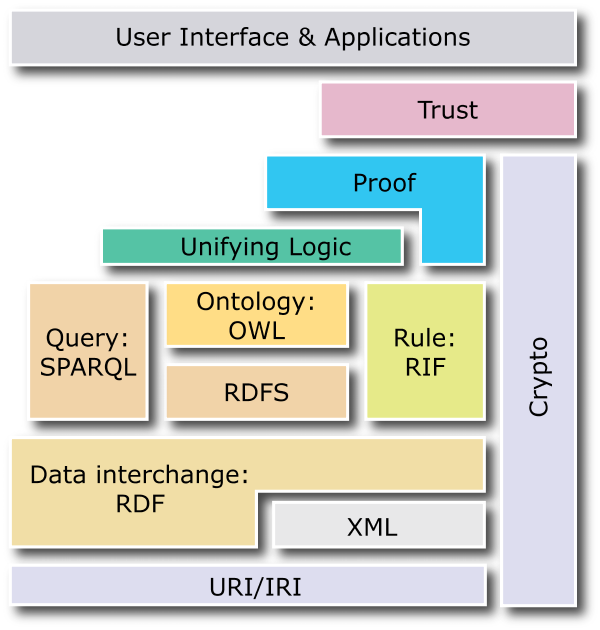
\includegraphics[width=180px]{imgs/Semantic_Web_Stack0.png}
% 	    \caption{The Semantic Web Stack}
% 	\end{figure}
% \end{frame}

\begin{frame}
	\frametitle{The Semantic Web Stack}
	L'insieme delle tecnologie impiegate nel Web Semantico 
	costituisce il \emph{Semantic Web Stack}.
	
	Tratteremo la gran parte di queste.
	
	\begin{figure}
	    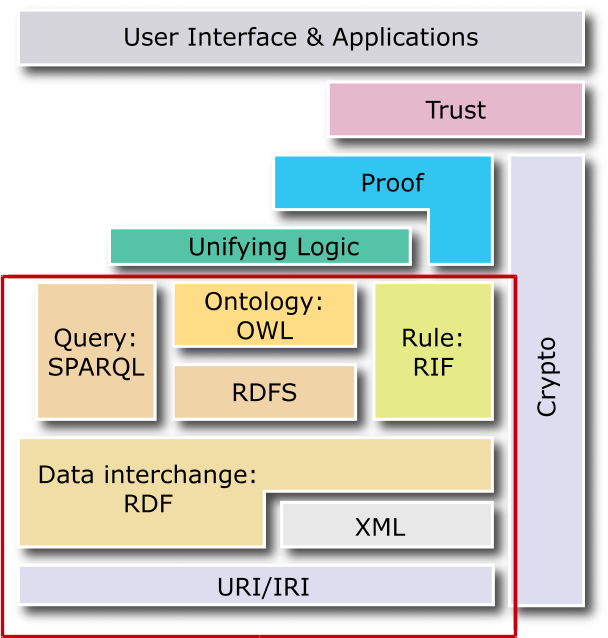
\includegraphics[width=180px]{imgs/Semantic_Web_Stack0all.png}
	    \caption{The Semantic Web Stack} 
	\end{figure}
\end{frame}

\begin{frame}
	\frametitle{URI/IRI}
	
	\begin{itemize}
	  \item \emph{Uniform Resource Identifiers} (URI) - RFC3986
	  \item \emph{Internationalized Resource Identifiers (IRIs)} (IRI) - RFC3987
	\end{itemize}	
	
	Nel Web Semantico le IRI servono ad \emph{indicare} oggetti di qualsiasi
	natura, concreti o astratti.
	
	\begin{figure}
	    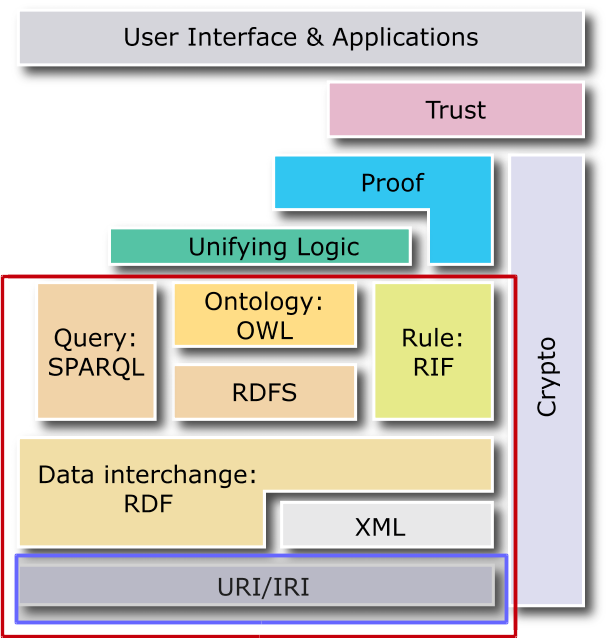
\includegraphics[width=180px]{imgs/Semantic_Web_Stack_uri.png}
	    \caption{The Semantic Web Stack} 
	\end{figure}
\end{frame}

\begin{frame}[fragile]
	\frametitle{Uniform Resource Identifier (URI)}
	La specifica \emph{Uniform Resource Identifier (URI)} ingloba
	le nozioni di Uniform Resource Name e Uniform Resource Locator
	ed \`e definita nell'RFC 3986.
	\vspace{\baselineskip}
	
	La \emph{grammatica} delle URI \`e espressa usando la notazione
	\emph{Augmented BNF for Syntax Specifications (ABNF)}, definita
	nell'RFC 2234. 
	\vspace{\baselineskip}

	I simboli terminali \tt{ALPHA} e \tt{DIGIT} indicano rispettivamente
	lettere e numeri disponibili nell'encoding \tt{US-Ascii}.
	\vspace{\baselineskip}
	
	\`E previsto un meccanismo di \emph{percent-encoding} per utilizzare
	caratteri non in \tt{US-Ascii}.
	
	\begin{verbatim}
  pct-encoded = "%" HEXDIG HEXDIG	
	\end{verbatim}	
	
\end{frame}

\begin{frame}[fragile]
	\frametitle{URI - caratteri riservati}
	
	I caratteri riservati solitamente ricoprono la funzione di 
	separatori per delimitare le varie parti della URI.
	
	\begin{verbatim}
 reserved    = gen-delims / sub-delims
 
 gen-delims  = ":" / "/" / "?" / "#" / "[" / "]" / "@"

 sub-delims  = "!" / "$" / "&" / "'" / "(" / ")"
                  / "*" / "+" / "," / ";" / "=" 
                  

                  
	\end{verbatim}
	\vspace{\baselineskip}
	
\uncover<2->{
	Nel caso in cui si abbia la necessit\`a di usare caratteri riservati
	nel corpo di alcune parti della URI e non come separatori, \`e possibile
	farlo applicando il percent-encodind.
	\vspace{\baselineskip}
}

\phantom{
 	I caratteri che possono comparire all'interno delle parti di una URI
 	sono detti \emph{non riservati}. In alre parole, i caratteri non riservati
 	sono tutti i caratteri permessi in una URI ad esclusione di quelli riservati.
}	
\end{frame}

\begin{frame}[fragile]
	\frametitle{URI - caratteri riservati}
	
	I caratteri riservati solitamente ricoprono la funzione di 
	separatori per delimitare le varie parti della URI.
	
	\begin{verbatim}
 reserved    = gen-delims / sub-delims
 
 gen-delims  = ":" / "/" / "?" / "#" / "[" / "]" / "@"

 sub-delims  = "!" / "$" / "&" / "'" / "(" / ")"
                  / "*" / "+" / "," / ";" / "=" 
                  
 unreserved  = ALPHA / DIGIT / "-" / "." / "_" / "~"
                  
	\end{verbatim}
	\vspace{\baselineskip}
	
	Nel caso in cui si abbia la necessit\`a di usare caratteri riservati
	nel corpo di alcune parti della URI e non come separatori, \'e possibile
	farlo applicando il percent-encodind.
	\vspace{\baselineskip}

 	I caratteri che possono comparire all'interno delle parti di una URI
 	sono detti \emph{non riservati}. In alre parole, i caratteri non riservati
 	sono tutti i caratteri permessi in una URI ad esclusione di quelli riservati.	
\end{frame}

\begin{frame}[fragile]
	\frametitle{URI - componenti di una URI}
	
	La sintassi delle URI \`e definita come segue:
	
	\begin{verbatim}
  URI = scheme ":" hier-part [ "?" query ] [ "#" fragment ]

  hier-part   = "//" authority path-abempty
              / path-absolute
              / path-rootless
              / path-empty                  
	\end{verbatim}
	\vspace{\baselineskip}
	
	Riportiamo due esempi di uri.
	\vspace{\baselineskip}

	\begin{figure}
	    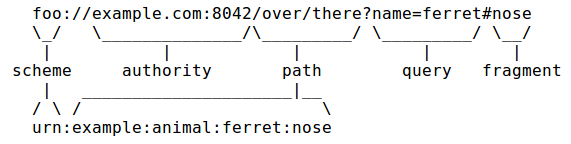
\includegraphics[width=250px]{imgs/uri-pieces.png}
	    \caption{Esempi di URI}
	\end{figure}
	
\end{frame}

\begin{frame}[fragile]
	\frametitle{URI - componenti - schema}
    Ogni URI inizia con uno \emph{schema}. Ogni schema identificana
    ulteriori restrizioni sintattiche nelle URI che vi ricadono.
    Alcuni schemi noti sono \tt{http}, \tt{mail}, \tt{tel}.\footnote{Un elenco
    esaustivo di URI scheme \`e disponibile alla pagina
    \url{http://www.iana.org/assignments/uri-schemes/uri-schemes.xhtml}.}
    \vspace{\baselineskip}
    
    Gli schemi hanno la seguente sintassi
    \begin{verbatim}
  scheme = ALPHA *( ALPHA / DIGIT / "+" / "-" / "." )
    \end{verbatim}    
\end{frame}

\begin{frame}[fragile]
	\frametitle{URI - componenti - authority}
	
	Molti URI scheme prevedono l'indicazione di una parte
	gerarchica denominata \emph{authority}. L'authority indica
	generalmente l'organizzazione responsabile delle risorse
	indicate dalla URI con l'authority in questione.
	Un esempio di authority (dello schema \tt{http}) \`e \tt{www.google.it}.
    \vspace{\baselineskip}
    
    La sintassi dell'authority \`e la seguente:
    \begin{verbatim}
  authority   = [ userinfo "@" ] host [ ":" port ]
    \end{verbatim}    

	\tt{userinfo} contiene il nome utente ed eventuali altre informazioni 
	necessarie per l'accesso alla risorsa indicata dalla URI (ad esempio la
	password).
    \begin{verbatim}
  userinfo    = *( unreserved / pct-encoded / sub-delims / ":" ) .
    \end{verbatim}    
    
    \tt{host} \`e fondamentalmente un indirizzo IP o un nome di
    dominio.\footnote{per le definizioni di \tt{IP-literal}, \tt{IPv4address} e
    \tt{reg-name} consultare lo RFC3986.}
    \begin{verbatim}
  host        = IP-literal / IPv4address / reg-name
    \end{verbatim}    
    
    Infine, \tt{port} \`e una indicazione sull'eventual porta di rete (vedi
    stack TCP/IP) per accedere al servizio.
    \begin{verbatim}
  port        = *DIGIT
    \end{verbatim}  
\end{frame}

\begin{frame}[fragile]
	\frametitle{URI - componenti - path}
	
	Il \emph{path} permette di specificare ulteriormente un percorso,
	usualmente gerarchico, per indicare una risorsa nell'amito dello
	schema e della eventuale authority. Un path \`e costituito da una
	sequenza di  \emph{segmenti} separati dal carattere \tt{/}.
	
	\begin{verbatim}
  URI = scheme ":" hier-part [ "?" query ] [ "#" fragment ]

  hier-part   = "//" authority path-abempty
              / path-absolute
              / path-rootless
              / path-empty                  

  path-abempty  = *( "/" segment ) ; begins with "/" or is empty
  path-absolute = "/" [ segment-nz *( "/" segment ) ] 
              ; begins with "/" but not "//"
  path-rootless = segment-nz *( "/" segment ) ; begins with a segment
  path-empty    = 0<pchar> ; zero characters  

  pchar = unreserved / pct-encoded / sub-delims / ":" / "@"  
	\end{verbatim}
	
	\begin{figure}
	    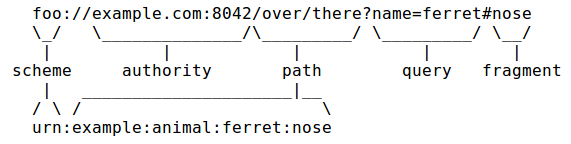
\includegraphics[width=250px]{imgs/uri-pieces.png}
	    \caption{Esempi di URI}
	\end{figure}
	
\end{frame}

\begin{frame}[fragile]
	\frametitle{URI - componenti - query}
	
	La \emph{query} \`e un componente opzionale non gerarchico che serve
	a specificare ulteriormente i parametri di indirizzamento della
	risorsa. Usualmente viene utilizzata per il passaggio dei parametri.
	
	\begin{verbatim}
  URI = scheme ":" hier-part [ "?" query ] [ "#" fragment ]

  query = *( pchar / "/" / "?" )
	\end{verbatim}
	
	\vspace{\baselineskip}
	
	\begin{figure}
	    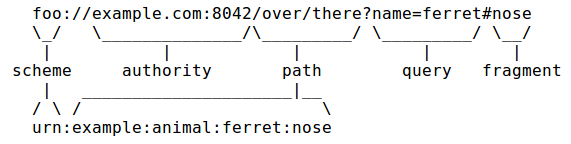
\includegraphics[width=250px]{imgs/uri-pieces.png}
	    \caption{Esempi di URI}
	\end{figure}
	
\end{frame}

\begin{frame}[fragile]
	\frametitle{URI - componenti - fragment}
	
	Il \emph{fragment} permette infine di indirizzare una risorsa
	\emph{secondaria} in riferimento ad una \emph{primaria}, ad esempio un
	frammento di una pagina web o un dato istante in un video.
	
	\begin{verbatim}
  URI = scheme ":" hier-part [ "?" query ] [ "#" fragment ]

  fragment    = *( pchar / "/" / "?" )
	\end{verbatim}
	
	\vspace{\baselineskip}
	
	\begin{figure}
	    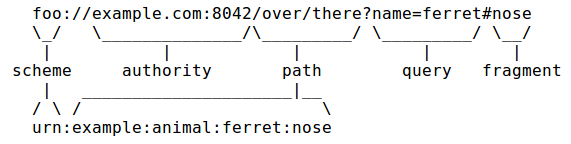
\includegraphics[width=250px]{imgs/uri-pieces.png}
	    \caption{Esempi di URI}
	\end{figure}
	
\end{frame}

\begin{frame}[fragile]
	\frametitle{Internationalized Resource Identifiers (IRIs)}

	La specifica delle \emph{Internationalized Resource Identifier (IRI)}
	estende quella delle URI con delle funzionali\`a per l'internazionalizzazione.
	\vspace{\baselineskip}
	 
	Una IRI \`e una sequenza di caratteri nell'\emph{Universal Character Set
	(Unicode/ISO 10646)}.
	
	La grammatica delle IRI pu\`o essere definita a partire da quella delle URI
	estendendo l'insieme dei caratteri non riservati per comprendere i caratteri
	nell'UCS.
	\begin{verbatim}
  iunreserved = ALPHA / DIGIT / "-" / "." / "_" / "~" / ucschar
	\end{verbatim}
	\vspace{\baselineskip}
	
	Per maggiori approfondimenti si veda l'RFC 3987.
\end{frame}

\section{XML}
\begin{frame}
	\frametitle{XML}
	 Il linguaggio \emph{eXtended Markup Language} (in breve \emph{XML})\footnote{\url{http://www.w3.org/XML/}} 
 \`e un liguaggio di marcatura basato su SGML ed \`e alla base del 
 linguaggio HTML (in particolare xHTML). XML \`e una specifica
 w3c, attualmente alla versione 1.1.\footnote{\url{http://www.w3.org/TR/2006/REC-xml11-20060816/}}
	
	\begin{figure}
	    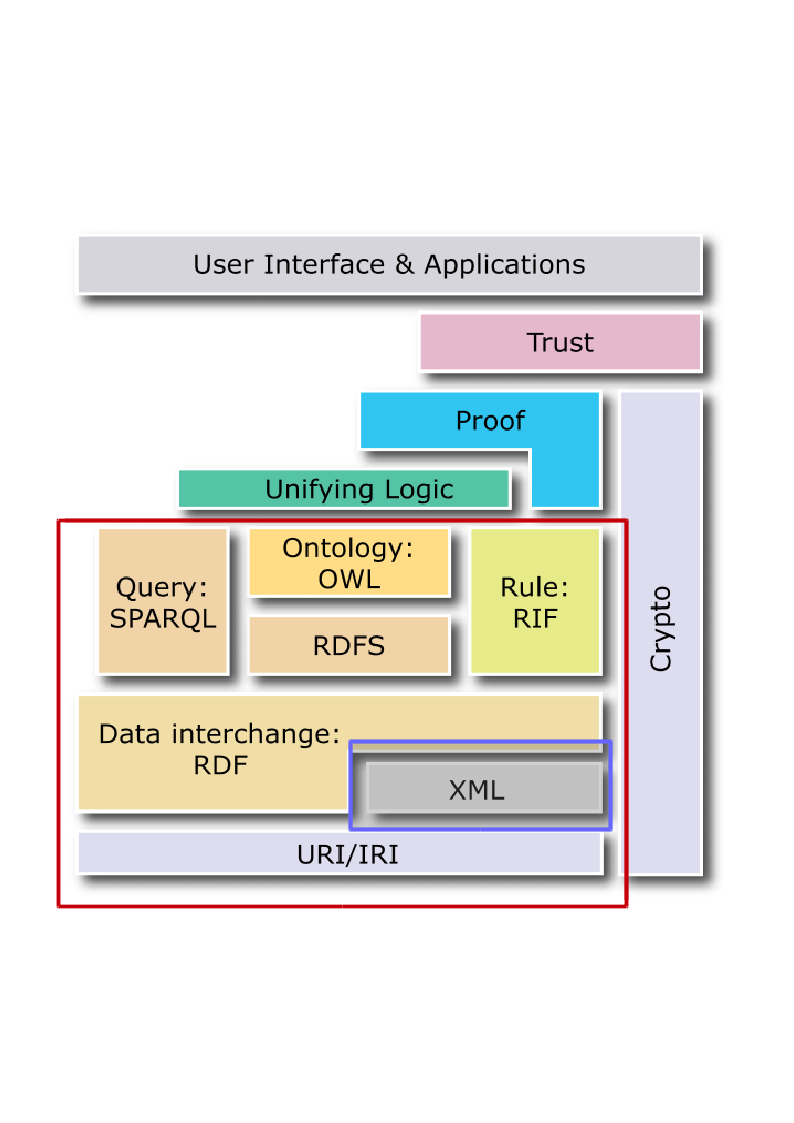
\includegraphics[width=180px]{imgs/Semantic_Web_Stack_xml.png}
	    \caption{The Semantic Web Stack} 
	\end{figure}
\end{frame}

\begin{frame}[fragile]
	\frametitle{Sintassi XML}
 Un documento XML \`e un documento di testo (codificato in UTF-8 o UTF16) 
 che rispetta le regole di produzione indicate nella specifica. 
 Un validatore per XML \`e disponibile al seguente indirizzo.
\begin{center}
\begin{small}
  \url{http://www.w3schools.com/xml/xml_validator.asp}
\end{small} 
\end{center}
 \vspace{\baselineskip}

 Escludendo le dichiarazioni, un documento XML \`e strutturato ad albero.
 Ogni nodo dell'albero pu\`o essere un \emph{elemento}, che pu\`o
 a sua volta contenere altri elementi, o un nodo di testo(TextNode).
 Segue un esempio di documento XML.\footnote{L'esempio \`e stato preso da
 \url{http://www.w3schools.com/xml/}.}
 \begin{verbatim}
  <?xml version="1.0" encoding="UTF-8"?>
  <note>
    <to>Tove</to>
    <from>Jani</from>
    <heading>Reminder</heading>
    <body>Don't forget me this weekend!</body>
  </note>  
 \end{verbatim}
\end{frame}

\begin{frame}[fragile]
 \frametitle{Sintassi XML - Elementi}

 
 Un elemento \`e caratterizzato da un \emph{element name}
 ed \`e delimitato da uno \emph{start tag} e un \emph{end tag},
 tranne nel caso di elementi vuoti.
 Un esempio di elemento con element name \texttt{myElement} \`e
 il seguente:
\begin{verbatim}
  <myElement>
    just a text content
  </myElement>
\end{verbatim}

 L'esempio seguente mostra un elemento vuoto.
\begin{verbatim}
  <emptyElement />
\end{verbatim}
  
 Ogni elemento pu\`o avere altri nodi come figli.
 Nell'esempio seguente viene mostrato un elemento 
 di tipo \texttt{myElement} con due nodi figli:
 un secondo element di tipo \texttt{elementChild}
 ed un nodo di testo.
\begin{verbatim}
  <myElement>
    <elementChild>child text content</elementChild>
    another text node
  </myElement>
\end{verbatim}
\end{frame}

\begin{frame}[fragile]
 \frametitle{XML - Attributi}
 Ogni elemento pu\`o avere degli \emph{attributi}.
 Un attributo di un elemento \`e una coppia nome-valore. 
 Nell'esempio seguente viene mostrato un elemento vuoto 
 di tipo \texttt{myElement} con un attributo \texttt{myAttr} 
 con valore \texttt{attrValue}.
\begin{verbatim}
  <myElement myAttribute="attrValue" />
\end{verbatim}
\end{frame}

\begin{frame}[fragile]
 \frametitle{XML - Struttura}
 Un \emph{documento XML} \`e suddiviso in due parti: prologo e 
 contenuto. Il prologo deve contenere la \emph{XML Declaration},
 mentre il contenuto \`e riservato agli elementi e deve contenere
 almeno un elemento (la radice).
 \vspace{\baselineskip}

 Riportiamo un esempio di documento XML:\footnote{Esempio da \url{http://www.w3schools.com/xml/xml_tree.asp} e lievemente modificato.}
\begin{small}
\begin{verbatim}
<?xml version="1.1" encoding="UTF-16"?> <!-- Prologo -->

<!-- Contenuto -->
<bookstore> <!-- Elemento radice -->
  <book category="COOKING">
    <title lang="en">Everyday Italian</title>
    <author>Giada De Laurentiis</author>
    <year>2005</year>
    <price>30.00</price>
  </book>
  <book category="WEB">
    <title lang="en">Learning XML</title>
    <author>Erik T. Ray</author>
    <year>2003</year>
    <price>39.95</price>
  </book>
</bookstore> 
\end{verbatim}
\end{small}
\end{frame}

\begin{frame}
 \frametitle{XML - Entit\`a}
 
 Le \emph{Entity References} sono particolari token che 
 vengono sostituiti con dei valori predefiniti (o dichiarati nel prologo)
 quando viene effettuato il parsing XML. Le entity references possono 
 comparire nei nodi di testo e come valore degli attributi degli elementi.
 \vspace{\baselineskip}
 
 Una entity reference inizia con il carttere \texttt{\&} e termina con \texttt{;}.
 Le entit\`a predefinite nel linguaggio XML sono le seguenti:
\[
 \begin{array}{|c|c|}
  \hline
    Entity Reference & Carattere \\
    \hline
    \mathtt{\&lt;} & \mathtt{<} \\
    \mathtt{\&gt;} & \mathtt{>} \\
    \mathtt{\&amp;} & \mathtt{\&}\\ 
    \mathtt{\&apos;} & \mathtt{'}\\
    \mathtt{\&quot;} & \mathtt{"}\\
  \hline
 \end{array}
\]
 \vspace{\baselineskip}

 Inoltre, \`e possibile fare riferimento ad uno specifico carattere
 mediante il codice attraverso il quale \`e identificato il carattere.
 In questo caso, si usa la sintassi \texttt{\&\#code;}, sostituendo 
 a \texttt{<code>} il codice unicode del carattere che si vuole inserire
 nel documento
 ad esempio, tutte le occorrenze di \texttt{\&\#8364;} verranno 
 sostituite con il carattere \texttt{\euro} durante il parsing di un 
 documento.
\end{frame}

\begin{frame}[fragile]
 \frametitle{XML - Entit\`a - Esempio}
 Riportiamo un esempio di documento XML che contiene delle entit\`a:
 \vspace{\baselineskip}
 
 \emph{Documento Originale}
\begin{small}
\begin{verbatim}
<?xml version="1.1" encoding="UTF-16"?>
<message>
  Non usare il tag &lt;euro /&gt; &#33;
</message>
\end{verbatim}
\end{small}

 \emph{Documento Interpretato} (33 \`e il codice unicode per \texttt{!})
\begin{small}
\begin{verbatim}
<?xml version="1.1" encoding="UTF-16"?>
<message>
  Non usare il tag <euro /> !
</message>
\end{verbatim}
\end{small} 
\end{frame}

\begin{frame}[fragile]
 \frametitle{XML - Document Type Declaration (1/3)}
Nel prologo di un documento XML pu\`o essere specificata una
\emph{Document Type Declaration}. 
\vspace{\baselineskip}

La document type declaration
specifica il \emph{tipo} di documento in termini di struttura
(tipi elementi, possibili annidamenti, attributi degli elementi).
\vspace{\baselineskip}

Riportiamo un esempio di documento xml che segue la specifica
(leggi \emph{\'e di tipo}) HTML5:\footnote{\url{http://www.w3.org/TR/html5/}}

\begin{small}
\begin{verbatim}
<?xml version="1.0" encoding="UTF-8" standalone="yes"?>
<!DOCTYPE html> <!-- the doctype declaration -->

<html>
  <head>
    <meta charset="UTF-8">
    <title>Title of the document</title>
   </head>
   <body>
     Content of the document......
   </body>
</html> 
\end{verbatim}
\end{small}
\vspace{\baselineskip}

NB: nei documenti HTML5 la XML Declaration pu\`o essere omessa.
\end{frame}

\begin{frame}[fragile]
 \frametitle{XML - Document Type Declaration (2/3)}
 
 La struttura pu\`o essere specificata:
 \vspace{\baselineskip}
 
 - usando i formati DTD e XML Schema;
 \vspace{\baselineskip}

 - internamente alla Document Type Declaration, ad esempio\footnote{Esempio da \url{http://www.w3schools.com/xml/xml_dtd_intro.asp} .}
\begin{small}
\begin{verbatim}
<!DOCTYPE note [
  <!ELEMENT note (to,from,heading,body)>
  <!ELEMENT to (#PCDATA)>
  <!ELEMENT from (#PCDATA)>
  <!ELEMENT heading (#PCDATA)>
  <!ELEMENT body (#PCDATA)>
]> 
\end{verbatim}
\end{small}

 - o come risorsa esterna al documento, ad esempio
\begin{small}
\begin{verbatim}
<!DOCTYPE note SYSTEM "note.dtd">
\end{verbatim}
\end{small}
\end{frame}

\begin{frame}[fragile]
 \frametitle{XML - Document Type Declaration (3/3)}
 Inoltre, all'interno della document type declaration possono essere
 specificate nuove entity refence.

\begin{small}
\begin{verbatim}
<!DOCTYPE rdf:RDF [
    <!ENTITY org "http://www.w3.org/ns/org#" >
    <!ENTITY dcterms "http://purl.org/dc/terms/" >
    <!ENTITY locn "http://www.w3.org/ns/locn#" >
    <!ENTITY foaf "http://xmlns.com/foaf/0.1/" >
    <!ENTITY owl "http://www.w3.org/2002/07/owl#" >
    <!ENTITY xsd "http://www.w3.org/2001/XMLSchema#" >
    <!ENTITY rdfs "http://www.w3.org/2000/01/rdf-schema#" >
    <!ENTITY geo "http://www.w3.org/2003/01/geo/wgs84_pos#" >
    <!ENTITY rdf "http://www.w3.org/1999/02/22-rdf-syntax-ns#" >
    <!ENTITY odt "http://www.dmi.unict.it/~longo/opendatatour/" >
    <!ENTITY event "http://purl.org/NET/c4dm/event.owl#" >
    <!ENTITY time "http://www.w3.org/2006/time#" >
    <!ENTITY cct "http://www.comune.catania.it/comunect.owl/" >
]>
\end{verbatim}
\end{small}
\end{frame}

\end{document}
